\newpage
\changeindent{0cm}
\section{数値実験}
\changeindent{2cm}

本章では, 提案手法の有効性を確認するために実施した 2 種類の実験について説明する. 提案手法の有効性は 2 種類の実験の結果を 2.4 節で説明した KG-BERT を用いた結果と比較することで確認した. \par

\subsection{データセット}

本研究では, Knowledge Graph として 2.5 節で説明した WN18RR を用いた. このデータセットは Head, Relation, Tail を Triple として保存している. WN18RR の Triple を比較手法の KG-BERT モデルの入力文と対応させるため, 先頭を ``[CLS]" トークンとして Head, Relation, Tail を ``[SEP]" トークンで区切ったトークン列を入力文とした. 表 \ref{dataset_example} に例を示す. \par
以下の 2 種類の実験では, WN18RR の Triple を訓練データ, 検証データ, テストデータとしてそれぞれ 8 : 1 : 1 に分割して用いた. 表 \ref{num} に WN18RR の内訳を示す. \par

\subsection{実験 1}

実験 1 では, 提案するモデルおよび学習方法の有効性を確認するため, 訓練データを用いて BERT を MLM で fine-tuning し, このモデルを用いてテストデータの Tail を予測させることでモデルの精度を確認した. \par
図 \ref{KG-MLM1} に実験 1 のモデル概略図を示す. BERT を MLM で fine-tuning したモデルに対して, Triple ``[CLS] Head [SEP] Relation [SEP] Tail [SEP]" における Tail の見出し語を ``[MASK]" トークンに置き換えた文 ``[CLS] Head [SEP] Relation [SEP] [MASK], Tail の説明文 [SEP]" を 1 つのシーケンスとして入力する. 図 \ref{KG-MLM} において ``Tail" を ``[MASK], description" とした場合である. これにより, ``[MASK]" トークンとなった Tail の見出し語を予測する. なお, 予測する Tail の見出し語の説明文をそのまま入力しているため, 通常想定される Tail 予測タスクより Tail の予測が容易である. \par
表 \ref{parameta_em} に比較手法の KG-BERT と実験 1 のパラメータを示す. なお, KG-BERT の eval batch size と max seq length はメモリ容量の都合上文献値とは異なっている. また, 表中の「- (ハイフン)」はそのモデルには必要のないパラメータを表している. \par

\begin{table}[t]
    \centering
    \caption{データセットをトークン列とした例}
    \label{dataset_example}
    \begin{tabular}{|c|} \hline
      [CLS]Head[SEP]Relation[SEP]Tail[SEP] \\ \hline \hline
      \begin{tabular}{c}
      [CLS]telephone set, electronic equipment that converts sound into electrical signals \\ that …[SEP]has part[SEP]telephone receiver, earphone that \\ converts electrical signals into sounds[SEP]
      \end{tabular}\\ \hline
      \begin{tabular}{c}
      [CLS]wireless telephone, a telephone that communicates by radio waves rather than \\ along cables[SEP]hypernym[SEP]telephone set, electronic equipment \\ that converts sound into electrical signals that …[SEP]
      \end{tabular}\\ \hline
      \begin{tabular}{c}
      [CLS]telephone receiver, earphone that converts electrical signals into \\ sounds[SEP]hypernym[SEP]phone, electro-acoustic transducer for \\ converting electric signals into sounds; …[SEP]
      \end{tabular}\\ \hline
      \vdots \\ \hline
    \end{tabular}
\end{table}

\begin{table}[t]
    \centering
    \caption{WN18RR の内訳}
    \label{num}
    \scalebox{1.0}{
    \begin{tabular}{|ccc|ccc|} \hline
        Entity & Relation & Triple & 訓練 & 検証 & テスト \\ \hline \hline
      40,943 & 11 & 93,003 & 86,835 & 3,034 & 3,134 \\ \hline
    \end{tabular}
    }
\end{table}

\begin{figure}[t]
    \centering
    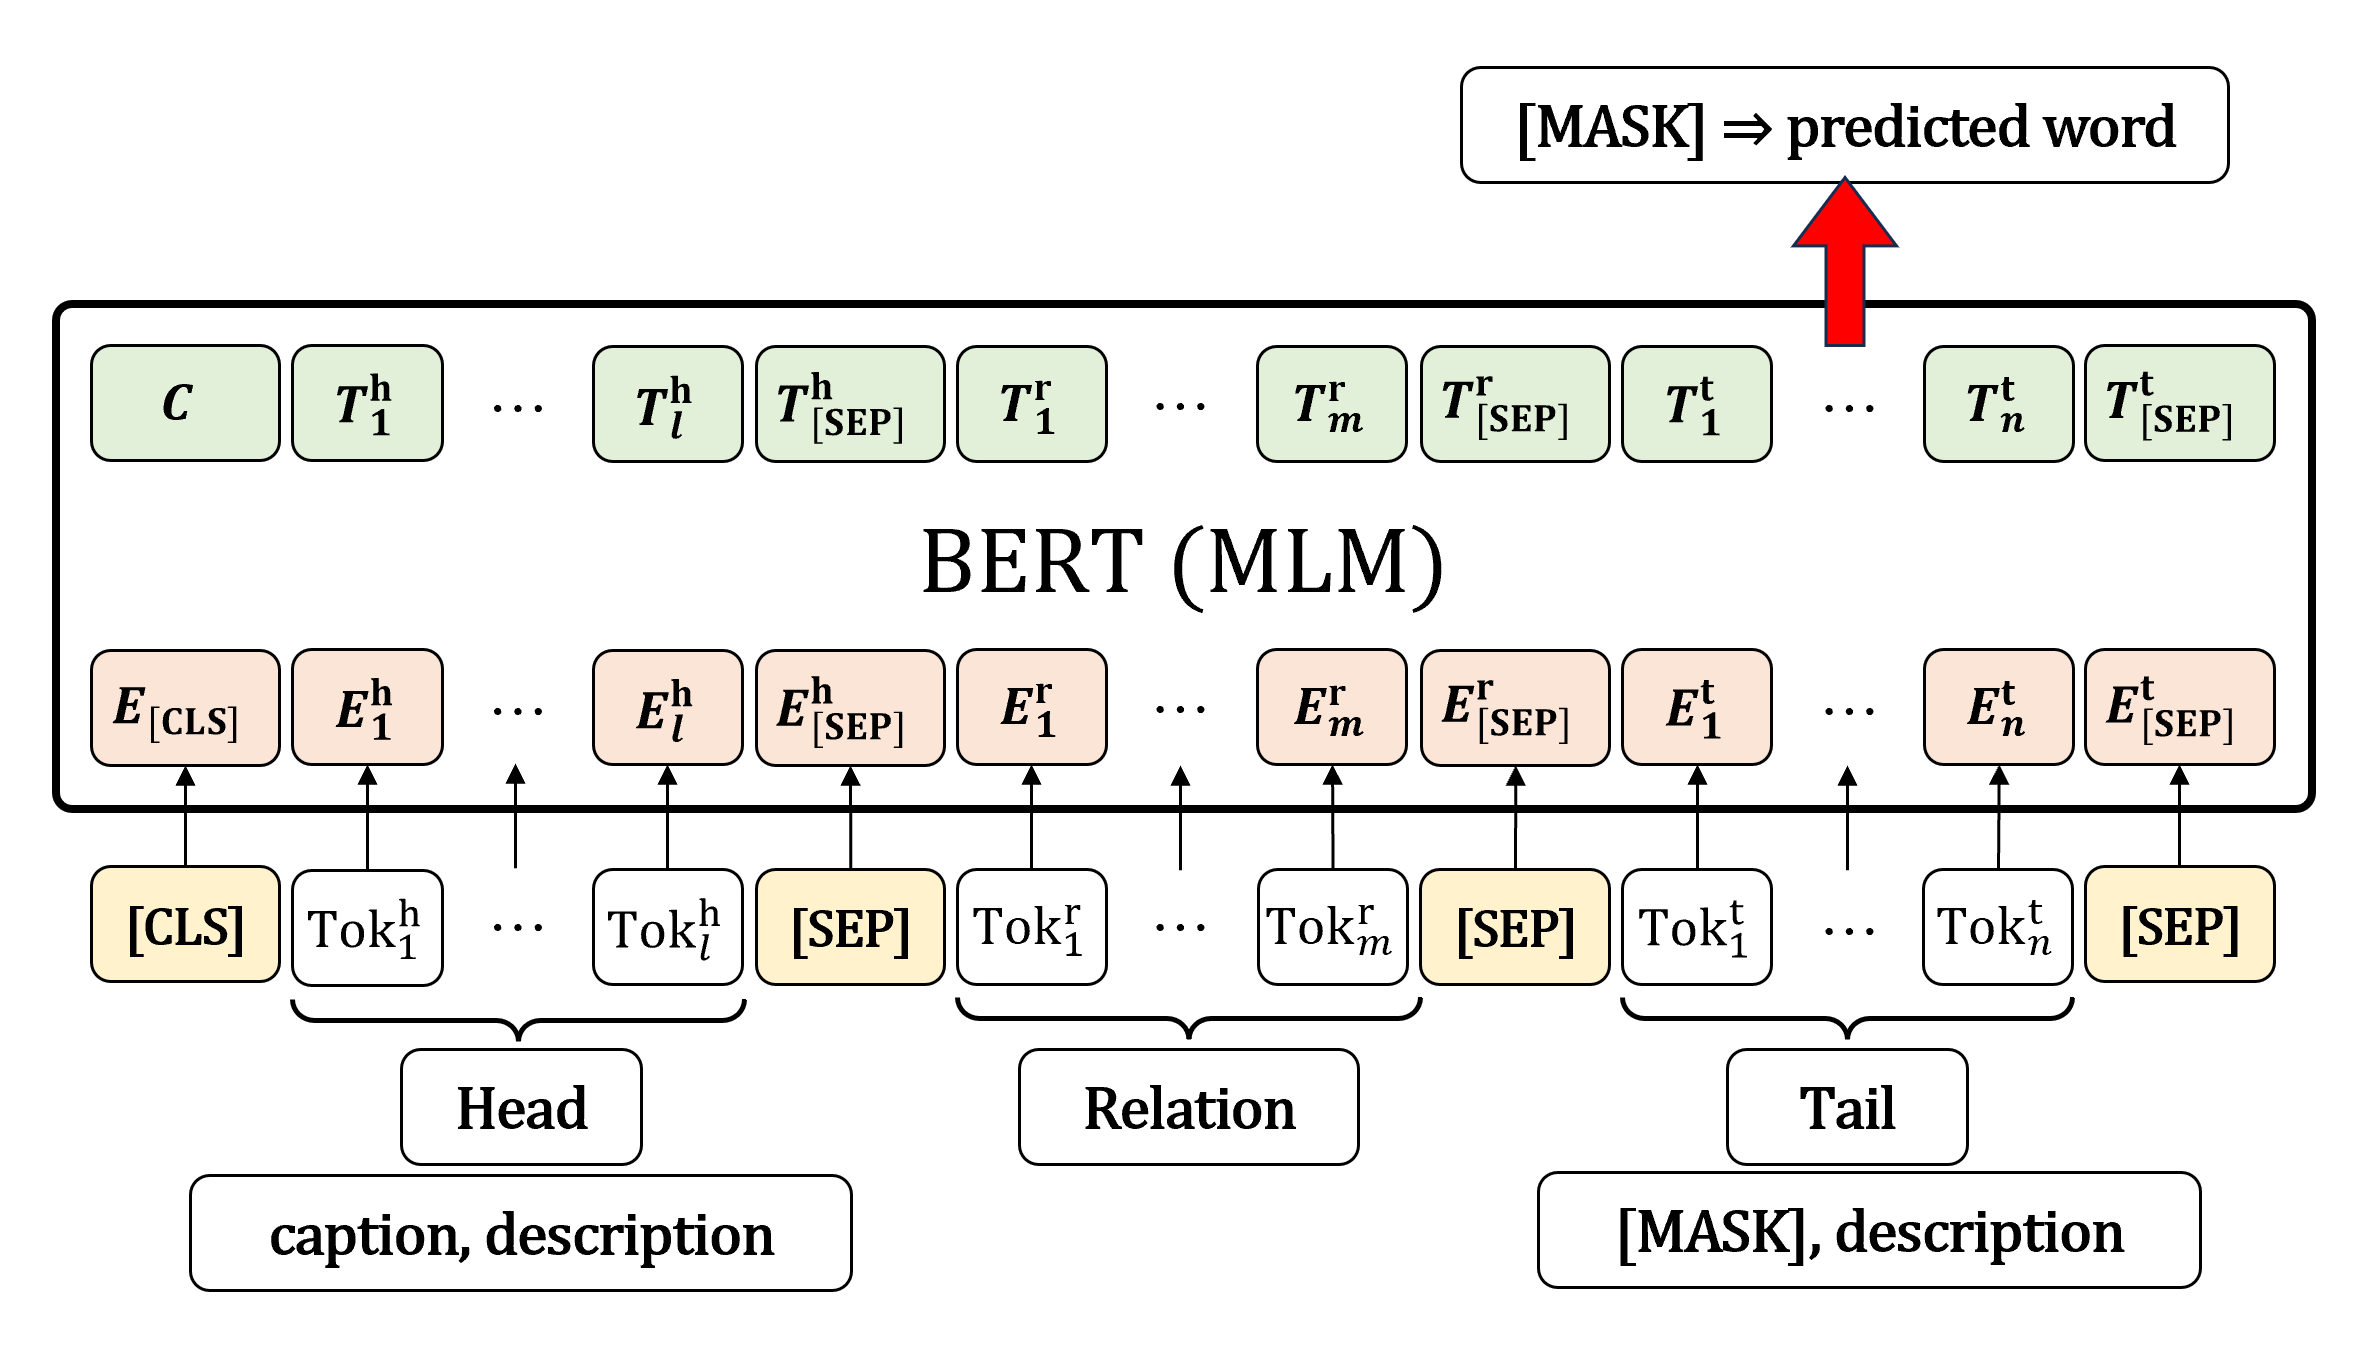
\includegraphics[width=16cm]{assets/KG-MLM1.png}
    \caption{実験 1 のモデル概略図}
    \label{KG-MLM1}
\end{figure}

\begin{figure}[t]
    \centering
    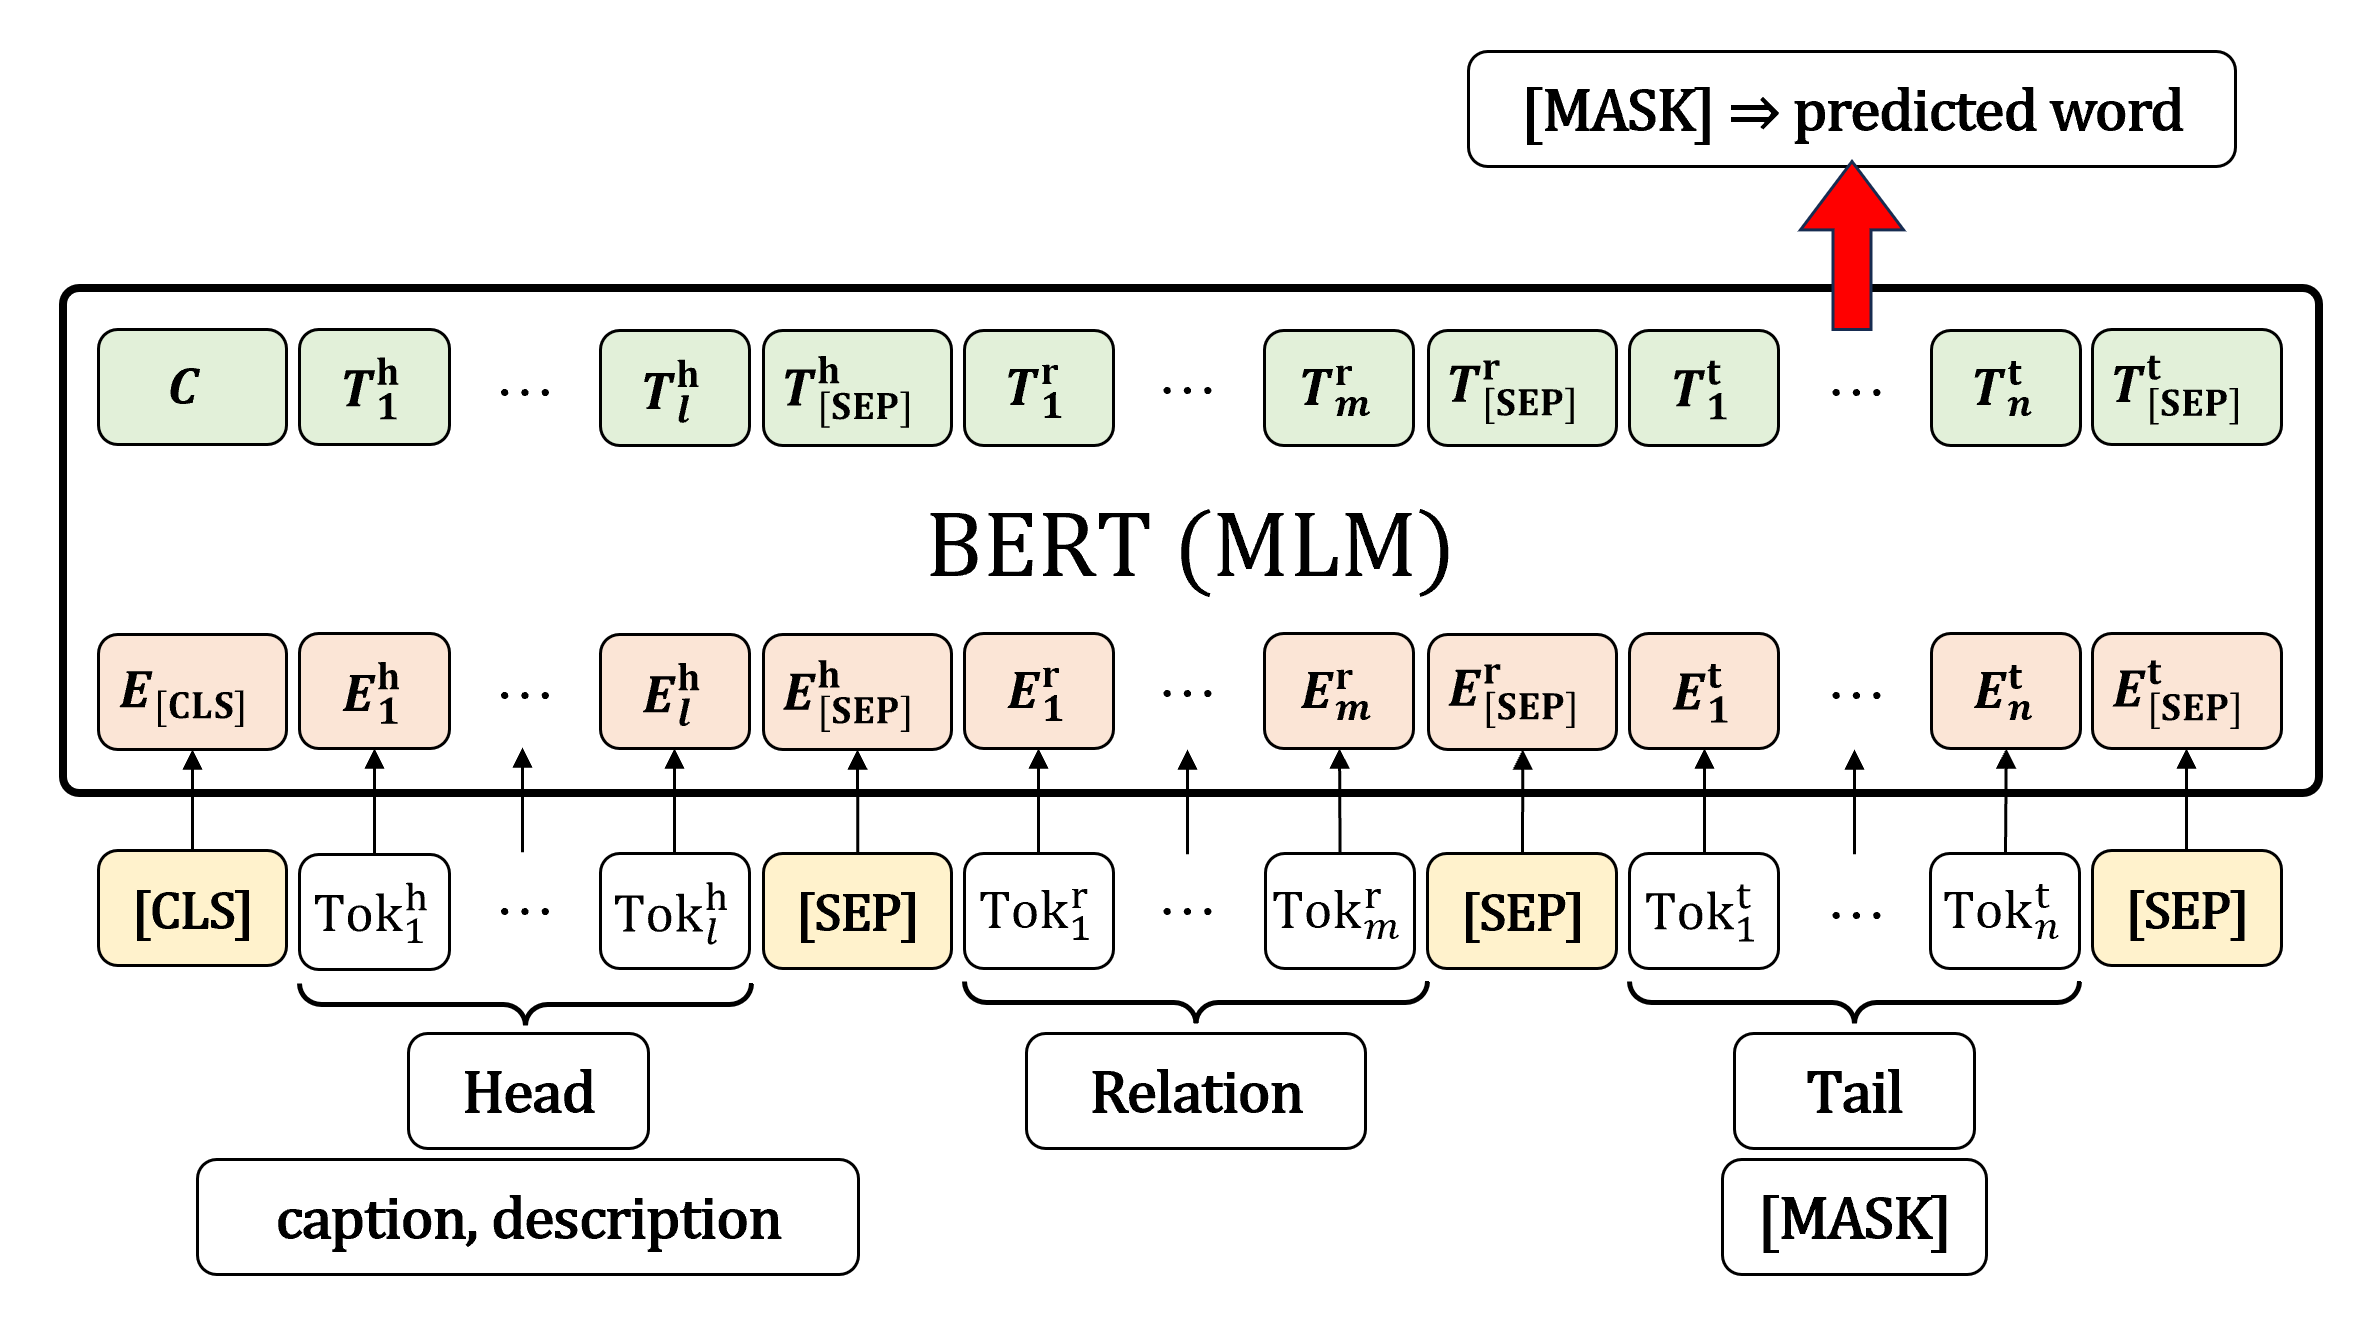
\includegraphics[width=16cm]{assets/KG-MLM2.png}
    \caption{実験 2 のモデル概略図}
    \label{KG-MLM2}
\end{figure}

\begin{table}[t]
    \centering
    \caption{KG-BERT と実験 1, 2 のパラメータ}
    \label{parameta_em}
    \scalebox{1.0}{
    \begin{tabular}{|c|c|c|} \hline
        パラメータ&KG-BERT (文献値)&実験 1, 2 \\ \hline \hline
        leaning rate&$5.0 \times 10^{-5}$&$5.0 \times 10^{-5}$\\
        mask probability&-&0.15\\\
        batch size&32&32\\
        eval batch size&128 (5000)&-\\
        max seq length&32 (50)&128\\
        epoch &5&20\\ \hline
    \end{tabular}
    }
\end{table}

\subsection{実験 2}

実験 2 では, 提案するモデルおよび学習方法の有効性を確認するため, 訓練データを用いて BERT を MLM で fine-tuning し, このモデルを用いてテストデータの Tail を予測させることでモデルの精度を確認した. なお, 実験 1 では Tail 予測のヒントとして Tail の説明文も入力していたのに対し, 実験 2 では Tail の説明文を入力しないものとする. \par
図 \ref{KG-MLM2} に実験 2 のモデル概略図を示す. 実験 1 の入力文 ``[CLS] Head [SEP] Relation [SEP] [MASK], Tail の説明文 [SEP]" における Tail の説明文を除去した文 ``[CLS] Head [SEP] Relation [SEP] [MASK] [SEP]" を 1 つのシーケンスとして入力する. この場合, 図 \ref{KG-MLM} における ``Tail" は ``[MASK]" のみとなる. これにより, ``[MASK]" トークンとなった Tail の見出し語を予測する. なお, 予測する Tail の見出し語の説明文は入力していないため, Head と Relation の情報のみを用いて Tail を予測する形となる. \par
実験 2 のパラメータは実験 1 と同様であり, 表 \ref{parameta_em} に示している. \par

\subsection{評価指標}

評価指標として Mean Reciprocal Rank (MRR), Hits@$k$, Filtered MRR, Filtered Hits@$k$ を用いる. 予測結果の $r$ 番目に正解があるとき, その順位 $r$ のことを Rank と呼ぶ. ${\rm |T|}$ を Triple 数, ${r}_{i}$ を Triple$_{i}$ における正解 Tail の Rank とすると, MRR は (\ref{MRR}) 式で表される. 
\begin{equation}
    {\rm MRR} = \frac{1}{\rm |T|} \sum^{\rm |T|}_{i=1} \frac{1}{r_{i}}
    \label{MRR}
\end{equation}
Hits@$k$ は, Tail 予測において上位 $k$ 個以内に正解の要素が出力されている割合を表す. このとき, あるテスト Triple の正解 Tail より予測結果の上位にそのテスト Triple と同じ Head と Relation をもつ Triple の Tail が存在する場合, その分低くランク付けされる. そこで, テスト Triple と同じ Head と Relation をもつ Triple の Tail を予測結果から除去してランク付けをする. この Rank を Filtered Rank とする. 表 \ref{filltered_Rank} に Filtered Rank の例を示す. 表 \ref{filltered_Rank} において, テスト Triple が (Head, Relation, Word $r$) で, データとして Triple (Head, Relation, Word 2), (Head, Relation, Word 4) の 2 つが存在するとき, Rank を 2 つ繰り上げることで Filtered Rank を得る. Filtered Rank によって計算される MRR, Hits@$k$ をそれぞれ Filtered MRR, Filtered Hits@$k$ とする. 本研究では $k=1, 3, 10$ で評価した. MMR, Hits@$k$, Filtered MRR, Filtered Hits@$k$ はすべて値が大きいと推定精度が良いと判断される. \par
ここで, 本実験と KG-BERT の Rank の所得方法について説明する. 本実験では, ``[MASK]" トークンに置き換えた箇所の単語を上位 300 位まで予測し, 正解 Tail がある順位を Rank とする. 予測できなかった Tail の Rank は Entity 数である 40,943 とする. KG-BERT では, 負例の Triple はある正例の Triple の Tail を他の Entity に置き換えて作成される. それらの Triple をそれぞれ BERT に入力する. これにより, 入力した Triple が正例である確率値を得る. このときに得られた値の降順に基づき, 正例の Triple とそれによって作成された複数の負例の Triple に対して順位付けをし, 得られた正例の Triple の順位を Rank とする. \par

\begin{table}[t]
    \centering
    \caption{Filtered Rank の例}
    \label{filltered_Rank}
    \scalebox{1.0}{
    \begin{tabular}{|c|c|cc|c|} \hline
      Triple&Rank&\multicolumn{2}{|c|}{Tail 予測結果}& Filtered Rank \\ \hline \hline
      &1&Word 1&&1 \\ \hline
      存在&2&Word 2&除去& - \\ \hline
      &3&Word 3&&2 \\ \hline
      存在&4&Word 4&除去& - \\ \hline
      &\vdots & \vdots&& \vdots \\ \hline
      正解&$r$ &Word $r$ && $r-2$ \\ \hline
    \end{tabular}
    }
\end{table}

\subsection{実験結果}

表 \ref{result} に KG-BERT と実験 1, 2 の結果を示す. KG-BERT は本実験と Tail 予測方法が異なるため単純な比較はできないが, 参考として文献値と再現実験の 2 つの結果を示している. 表中の「- (ハイフン)」は文献 \cite{KG-BERT} に記載されていなかったことを表している. \par

\begin{table}[t]
    \centering
    \caption{KG-BERT と実験 1, 2 の結果}
    \label{result}
    \scalebox{1.0}{
    \begin{tabular}{|c|cccc|} \hline
        &\multicolumn{4}{|c|}{WN18RR}\\
        モデル&MRR&Hits@1&Hits@3&Hits@10\\ \hline \hline
        KG-BERT (文献値)&-&-&-&52.4\\
        KG-BERT (再現実験)&0.25&12.41&29.44&51.85\\ \hline
        実験 1&0.546&52.55&56.16&57.79\\
        実験 1 (Filtered)&0.550&52.81&56.38&57.82\\ \hline
        実験 2&0.168&10.94&19.37&27.95\\
        実験 2 (Filtered)&0.169&11.04&19.66&28.05\\ \hline
    \end{tabular}
    }
\end{table}

表 \ref{result} より, 実験 1 ではすべての評価指標において KG-BERT の結果を上回る結果が得られた. これにより, Tail 予測に BERT の MLM を利用することの有効性が確認できた. しかし, 通常想定される Tail 予測タスクより Tail の予測が容易であるため, KG-BERT と単純な比較はできない. また, Filtered MRR, Filtered Hits@$k$ について MRR, Hits@$k$ と比較するとその値の変化は微細な範囲にとどまった. \par
実験 2 では Hits@$1$ において KG-BERT と同程度の結果が得られたが, 他の評価指標においては下回る結果となった. また, Filtered MRR, Filtered Hits@$k$ については実験 1 と同様に MRR, Hits@$k$ より少し向上したがほとんど変化していなかった. \par

\subsection{考察}

本節では Triple を (``Head の見出し語, その説明文", ``Relation", ``Tail の見出し語, その説明文") とし, Tail の見出し語を太字で表す. \par
Tail 予測の結果について本実験と KG-BERT の再現実験を比較する. \par
実験 1 でテスト Triple (``position, the particular portion of space occupied …", ``hypernym", ``\textbf{point}, the precise location of something; a spatially limited location; ``she walked to a point where she could survey the whole street"") の見出し語 ``point" を ``[MASK]" に置き換えて Tail を予測すると, 提案手法では ``point (地点)" を予測して正解したのに対し, KG-BERT では ``situation (状況)" を予測していた. これは Tail の見出し語の説明文に ``point" が含まれていることが予測に影響を与えたと考えられる. そのため, Tail の説明文の情報が結果に大きく影響することがわかった. \par
実験 2 でテスト Triple (``evidence, an indication that makes something evident; …", ``hypernym", ``\textbf{indication}, something that serves to indicate or suggest; …") の見出し語 ``indication" とその説明文を ``[MASK]" に置き換えて Tail を予測すると, 提案手法では ``indication (指示)" を予測して正解したのに対し, KG-BERT では ``averment (喚起)" を予測していた. これは Head の見出し語の説明文に ``indication" が含まれていることが予測に影響を与えたと考えられる. このような Head の見出し語の説明文に Tail の情報を含む Triple に対して提案手法は有効であることがわかった.\par
本実験の Tail 予測結果について考察する. \par
実験 1 でテスト Triple (``signer, someone who can use sign language to communicate", ``hypernym", ``\textbf{communicator}, a person who communicates with others") の見出し語 ``communicator" を ``[MASK]" に置き換えて Tail を予測すると, ``communicate" を予測していた. ``communicator (コミュニケーションをとる人)" と ``communicate (コミュニケーションをとる)" は派生語であり意味が近い単語として捉えることができる. また, 実験 2 でテスト Triple (``existence, the state or fact of existing; ``a point of view gradually coming into being"; ``laws in existence for centuries"", ``derivationally related form", ``\textbf{existent}, presently existing in fact and not merely potential or possible; …") の見出し語 ``existent" を ``[MASK]" に置き換えて Tail を予測すると, ``existence" を予測していた. 同様に ``existent (現存する)" と ``existence (存在)" は派生語であり意味が近い単語として捉えることができる. このように, 実験 1, 2 において正解 Tail の派生語であり意味が近い単語を予測できる可能性があることがわかる. しかし, 本実験ではこのような予測結果に対して間違いであると評価している場合がある. そこで, 予測結果が正解 Tail の派生語であり意味が近い単語であることを考慮する評価方法を追加することを今後検討する. \par
実験 1, 2 の Filtered MRR, Filtered Hits@$k$ においてどちらも MRR, Hits@$k$ と比較するとその値の変化は微細な範囲にとどまった. Filtered MRR, Filtered Hits@$k$ について考察する. \par
実験 1 では, 予測する Tail の説明文を入力していることにより Head と Relation が同じ他の Triple の Tail を予測する可能性が少ないと考えられる. 実験 2 では, テスト Triple (``vanish, become invisible or unnoticeable; ``The effect vanished when day broke"", ``derivationally related form", ``\textbf{disappearence}, the event of passing out of sight") の見出し語 ``disappearence" とその説明文を ``[MASK]" に置き換えて Tail を予測すると, 予測結果 2 番目に ``fade (次第に消える)" があり, ``disappearence (消滅)" を予測できていない例があった. なお, 訓練データ内に テスト Triple の Head と Relation が同じで Tail が ``fade" の Triple (``vanish, become invisible or unnoticeable; ``The effect vanished when day broke"", ``derivationally related form", ``\textbf{fade}, gradually ceasing to be visible") が存在している. このように, 訓練データ内にある Triple の影響で Tail を予測できないことが MRR, Hits@$k$ と Filtered MRR, Filtered Hits@$k$ の値に変化がない原因であると考えられる. \par
本研究では, MLM の出力は BERT に登録されている単語すべてが候補となっているため, WN18RR データセット内に Entity として存在しない単語も出力される可能性がある. そこで, MLM の出力候補を WN18RR データセット内の Entity のみに限定したモデルの作成を検討し, Tail の予測精度の向上を目指す. \par
